\documentclass[10pt,a4paper,fleqn]{article}
\setlength{\oddsidemargin}{-1.4mm}
\setlength{\evensidemargin}{-1.4mm}
\setlength{\textwidth}{162mm}
\setlength{\topmargin}{-12mm}
\setlength{\textheight}{249mm}
\usepackage{amsmath,amssymb,bm,booktabs,array}
\usepackage{xcolor,graphicx,tikz,pgfplots}
\usepackage{url}
% Clickable, breakable URLs using pdfTeX primitives; no hyperref dependency.
\let\plainurl\url
\renewcommand{\url}[1]{\ifdefined\pdfstartlink\leavevmode\pdfstartlink attr{/Border [0 0 0]} user{/Subtype /Link /A << /S /URI /URI (\pdfescapestring{#1}) >>}\plainurl{#1}\pdfendlink\else\plainurl{#1}\fi}
\pgfplotsset{compat=1.18}
\newif\ifmarked
\markedfalse
\definecolor{revisionblue}{RGB}{18,61,130}
\newcommand{\rev}[1]{{\ifmarked\color{revisionblue}\else\color{black}\fi #1}}
\newenvironment{revision}{\begingroup\ifmarked\color{revisionblue}\else\color{black}\fi\nobreak\ignorespaces}{\par\endgroup}
\newcommand{\Eavg}{\overline{\mathcal E}_h}
\newcommand{\Cstep}{\mathcal C}
\newcommand{\Rstep}{\mathcal R}
\newcommand{\mean}[1]{\overline{#1}}
\setlength{\textfloatsep}{14pt plus 3pt minus 2pt}
\setlength{\intextsep}{14pt plus 3pt minus 2pt}
\renewcommand{\topfraction}{0.9}
\renewcommand{\textfraction}{0.08}
\renewcommand{\floatpagefraction}{0.75}
\raggedbottom
\setlength{\emergencystretch}{1em}
\pagestyle{empty}
\makeatletter
\newlabel{eq:ch}{{1}{2}{}{equation.1}{}}
\newlabel{eq:energy}{{2}{2}{}{equation.2}{}}
\newlabel{eq:structure}{{3}{2}{}{equation.3}{}}
\newlabel{eq:step}{{4}{3}{}{equation.4}{}}
\newlabel{eq:fit}{{5}{3}{}{equation.5}{}}
\newlabel{eq:ridge}{{6}{3}{}{equation.6}{}}
\newlabel{eq:candidate}{{7}{3}{}{equation.7}{}}
\newlabel{eq:discreteenergy}{{8}{3}{}{equation.8}{}}
\newlabel{eq:derivatives}{{9}{3}{}{equation.9}{}}
\newlabel{eq:massproj}{{10}{4}{}{equation.10}{}}
\newlabel{eq:accept}{{11}{4}{}{equation.11}{}}
\newlabel{eq:backtrack}{{12}{4}{}{equation.12}{}}
\newlabel{eq:descent}{{13}{4}{}{equation.13}{}}
\newlabel{eq:galerkinenergy}{{14}{5}{}{equation.14}{}}
\newlabel{eq:galerkinlaw}{{15}{5}{}{equation.15}{}}
\newlabel{eq:pidmd}{{16}{5}{}{equation.16}{}}
\newlabel{eq:adaptive}{{17}{5}{}{equation.17}{}}
\newlabel{eq:initial}{{18}{6}{}{equation.18}{}}
\newlabel{eq:errors}{{19}{7}{}{equation.19}{}}
\newlabel{eq:structureerror}{{20}{7}{}{equation.20}{}}
\newlabel{eq:violation}{{21}{7}{}{equation.21}{}}
\newlabel{eq:rectangles}{{22}{7}{}{equation.22}{}}
\newlabel{tab:accuracy}{{1}{8}{}{table.1}{}}
\newlabel{tab:epsilon}{{2}{10}{}{table.2}{}}
\newlabel{tab:mobility}{{3}{10}{}{table.3}{}}
\newlabel{tab:long}{{4}{11}{}{table.4}{}}
\newlabel{tab:timing}{{5}{12}{}{table.5}{}}
\newlabel{eq:cost}{{23}{13}{}{equation.23}{}}
\newlabel{tab:convergence}{{6}{13}{}{table.6}{}}
\newlabel{tab:teacher}{{7}{14}{}{table.7}{}}
\newlabel{tab:finer}{{8}{15}{}{table.8}{}}
\newlabel{tab:crossgrid}{{9}{15}{}{table.9}{}}
\newlabel{tab:deterministic}{{10}{15}{}{table.10}{}}
\newlabel{tab:hyper}{{11}{17}{}{table.11}{}}
\newlabel{tab:shifts}{{12}{17}{}{table.12}{}}
\newlabel{eq:fixedfilterlimit}{{24}{18}{}{equation.24}{}}
\makeatother
\begin{document}
\setcounter{figure}{7}
\begin{figure}[htbp]\centering
\begin{tikzpicture}
\begin{axis}[width=.46\textwidth,height=5.4cm,grid=major,grid style={gray!15},tick label style={font=\footnotesize},label style={font=\small},xlabel={$t$},ylabel={Relative field error},title={(a)},title style={font=\small},legend style={font=\scriptsize,draw=none},legend style={at={(0.97,0.50)},anchor=east},ymode=log]
\addplot[thick,solid,mark=*,mark size=2pt,mark options={solid},mark repeat=7,blue!65!black] coordinates {(1e-07,2.60495323e-06) (6e-07,1.5626332e-05) (1.1e-06,2.86420687e-05) (1.6e-06,4.16521687e-05) (2.1e-06,5.4656637e-05) (2.6e-06,6.76554787e-05) (3.1e-06,8.06486989e-05) (3.6e-06,9.36363027e-05) (4.1e-06,0.000106618295) (4.6e-06,0.000119594681) (5.1e-06,0.000132565466) (5.6e-06,0.000145530655) (6.1e-06,0.000158490253) (6.6e-06,0.000171444265) (7.1e-06,0.000184392696) (7.6e-06,0.000197335551) (8.1e-06,0.000210272835) (8.6e-06,0.000223204553) (9.1e-06,0.00023613071) (9.6e-06,0.000249051311) (1.01e-05,0.000261966362) (1.06e-05,0.000274875866) (1.11e-05,0.000287779829) (1.16e-05,0.000300678256) (1.21e-05,0.000313571153) (1.26e-05,0.000326458523) (1.31e-05,0.000339340372) (1.36e-05,0.000352216704) (1.41e-05,0.000365087526) (1.46e-05,0.00037795284) (1.51e-05,0.000390812654) (1.56e-05,0.000403666971) (1.61e-05,0.000416515796) (1.66e-05,0.000429359134) (1.71e-05,0.00044219699) (1.76e-05,0.000455029369) (1.81e-05,0.000467856276) (1.86e-05,0.000480677716) (1.91e-05,0.000493493693) (1.96e-05,0.000506304213) (2.01e-05,0.000519109279) (2.06e-05,0.000531908898) (2.11e-05,0.000544703074) (2.16e-05,0.000557491811) (2.21e-05,0.000570275114) (2.26e-05,0.000583052989) (2.31e-05,0.00059582544) (2.36e-05,0.000608592471) (2.41e-05,0.000621354088) (2.46e-05,0.000634110296) (2.51e-05,0.000646861098) (2.56e-05,0.000659606501) (2.61e-05,0.000672346508) (2.66e-05,0.000685081124) (2.71e-05,0.000697810354) (2.76e-05,0.000710534203) (2.81e-05,0.000723252676) (2.86e-05,0.000735965777) (2.91e-05,0.00074867351) (2.96e-05,0.000761375882) (3.01e-05,0.000774072895) (3.06e-05,0.000786764556) (3.11e-05,0.000799450868) (3.16e-05,0.000812131836) (3.21e-05,0.000824807465) (3.26e-05,0.00083747776) (3.31e-05,0.000850142726) (3.36e-05,0.000862802366) (3.41e-05,0.000875456685) (3.46e-05,0.000888105689)};
\addlegendentry{Safeguarded}
\addplot[thick,dashed,mark=square*,mark size=2pt,mark options={solid},mark repeat=7,orange!85!black] coordinates {(1e-07,1.21535353e-05) (6e-07,7.29983458e-05) (1.1e-06,0.000133972166) (1.6e-06,0.000195075616) (2.1e-06,0.00025630932) (2.6e-06,0.000317673905) (3.1e-06,0.000379170004) (3.6e-06,0.000440798251) (4.1e-06,0.000502559286) (4.6e-06,0.000564453752) (5.1e-06,0.000626482294) (5.6e-06,0.000688645564) (6.1e-06,0.000750944217) (6.6e-06,0.000813378911) (7.1e-06,0.000875950308) (7.6e-06,0.000938659074) (8.1e-06,0.00100150588) (8.6e-06,0.0010644914) (9.1e-06,0.00112761632) (9.6e-06,0.00119088131) (1.01e-05,0.00125428706) (1.06e-05,0.00131783427) (1.11e-05,0.00138152362) (1.16e-05,0.00144535583) (1.21e-05,0.00150933158) (1.26e-05,0.00157345159) (1.31e-05,0.00163771658) (1.36e-05,0.00170212725) (1.41e-05,0.00176668434) (1.46e-05,0.00183138855) (1.51e-05,0.00189624063) (1.56e-05,0.00196124131) (1.61e-05,0.00202639132) (1.66e-05,0.00209169141) (1.71e-05,0.00215714233) (1.76e-05,0.00222274483) (1.81e-05,0.00228849966) (1.86e-05,0.0023544076) (1.91e-05,0.00242046939) (1.96e-05,0.00248668582) (2.01e-05,0.00255305766) (2.06e-05,0.00261958568) (2.11e-05,0.00268627069) (2.16e-05,0.00275311345) (2.21e-05,0.00282011478) (2.26e-05,0.00288727547) (2.31e-05,0.00295459632) (2.36e-05,0.00302207814) (2.41e-05,0.00308972175) (2.46e-05,0.00315752797) (2.51e-05,0.00322549762) (2.56e-05,0.00329363153) (2.61e-05,0.00336193054) (2.66e-05,0.00343039549) (2.71e-05,0.00349902722) (2.76e-05,0.00356782658) (2.81e-05,0.00363679443) (2.86e-05,0.00370593164) (2.91e-05,0.00377523905) (2.96e-05,0.00384471756) (3.01e-05,0.00391436803) (3.06e-05,0.00398419135) (3.11e-05,0.00405418841) (3.16e-05,0.0041243601) (3.21e-05,0.00419470732) (3.26e-05,0.00426523097) (3.31e-05,0.00433593197) (3.36e-05,0.00440681124) (3.41e-05,0.00447786968) (3.46e-05,0.00454910824)};
\addlegendentry{Unconstrained}
\addplot[thick,dashdotted,mark=triangle*,mark size=2pt,mark options={solid},mark repeat=7,teal!80!black] coordinates {(1e-07,1.63194911e-11) (6e-07,9.78510252e-11) (1.1e-06,1.79272757e-10) (1.6e-06,2.60584934e-10) (2.1e-06,3.41787765e-10) (2.6e-06,4.22881461e-10) (3.1e-06,5.03866212e-10) (3.6e-06,5.84742207e-10) (4.1e-06,6.65509742e-10) (4.6e-06,7.46168954e-10) (5.1e-06,8.26720115e-10) (5.6e-06,9.07163379e-10) (6.1e-06,9.87498992e-10) (6.6e-06,1.06772713e-09) (7.1e-06,1.147848e-09) (7.6e-06,1.22786178e-09) (8.1e-06,1.30776876e-09) (8.6e-06,1.38756906e-09) (9.1e-06,1.46726296e-09) (9.6e-06,1.54685061e-09) (1.01e-05,1.62633221e-09) (1.06e-05,1.70570801e-09) (1.11e-05,1.7849782e-09) (1.16e-05,1.86414296e-09) (1.21e-05,1.9432025e-09) (1.26e-05,2.02215699e-09) (1.31e-05,2.10100666e-09) (1.36e-05,2.17975173e-09) (1.41e-05,2.25839236e-09) (1.46e-05,2.33692876e-09) (1.51e-05,2.41536114e-09) (1.56e-05,2.4936897e-09) (1.61e-05,2.57191459e-09) (1.66e-05,2.65003612e-09) (1.71e-05,2.72805435e-09) (1.76e-05,2.80596951e-09) (1.81e-05,2.88378182e-09) (1.86e-05,2.96149147e-09) (1.91e-05,3.03909865e-09) (1.96e-05,3.11660358e-09) (2.01e-05,3.19400645e-09) (2.06e-05,3.2713074e-09) (2.11e-05,3.34850662e-09) (2.16e-05,3.42560434e-09) (2.21e-05,3.50260072e-09) (2.26e-05,3.57949602e-09) (2.31e-05,3.65629036e-09) (2.36e-05,3.73298394e-09) (2.41e-05,3.80957697e-09) (2.46e-05,3.88606961e-09) (2.51e-05,3.96246207e-09) (2.56e-05,4.03875451e-09) (2.61e-05,4.11494713e-09) (2.66e-05,4.19104014e-09) (2.71e-05,4.26703372e-09) (2.76e-05,4.34292801e-09) (2.81e-05,4.41872324e-09) (2.86e-05,4.49441961e-09) (2.91e-05,4.5700172e-09) (2.96e-05,4.6455163e-09) (3.01e-05,4.72091707e-09) (3.06e-05,4.79621965e-09) (3.11e-05,4.87142424e-09) (3.16e-05,4.94653101e-09) (3.21e-05,5.02154019e-09) (3.26e-05,5.09645195e-09) (3.31e-05,5.17126644e-09) (3.36e-05,5.24598383e-09) (3.41e-05,5.32060429e-09) (3.46e-05,5.39512804e-09)};
\addlegendentry{Six substeps}
\end{axis}
\end{tikzpicture}\hfill
\begin{tikzpicture}
\begin{axis}[width=.46\textwidth,height=5.4cm,grid=major,grid style={gray!15},tick label style={font=\footnotesize},label style={font=\small},xlabel={$t$},ylabel={$\alpha$},title={(b)},title style={font=\small},legend style={font=\scriptsize,draw=none},legend pos=north west,ymode=log]
\addplot[thick,densely dotted,mark=diamond*,mark size=2pt,mark options={solid},mark repeat=7,blue!65!black] coordinates {(1e-07,1.49011612e-08) (6e-07,1.49011612e-08) (1.1e-06,1.49011612e-08) (1.6e-06,1.49011612e-08) (2.1e-06,1.49011612e-08) (2.6e-06,1.49011612e-08) (3.1e-06,1.49011612e-08) (3.6e-06,1.49011612e-08) (4.1e-06,1.49011612e-08) (4.6e-06,1.49011612e-08) (5.1e-06,1.49011612e-08) (5.6e-06,1.49011612e-08) (6.1e-06,1.49011612e-08) (6.6e-06,1.49011612e-08) (7.1e-06,1.49011612e-08) (7.6e-06,1.49011612e-08) (8.1e-06,1.49011612e-08) (8.6e-06,1.49011612e-08) (9.1e-06,1.49011612e-08) (9.6e-06,1.49011612e-08) (1.01e-05,1.49011612e-08) (1.06e-05,1.49011612e-08) (1.11e-05,1.49011612e-08) (1.16e-05,1.49011612e-08) (1.21e-05,1.49011612e-08) (1.26e-05,1.49011612e-08) (1.31e-05,1.49011612e-08) (1.36e-05,1.49011612e-08) (1.41e-05,1.49011612e-08) (1.46e-05,1.49011612e-08) (1.51e-05,1.49011612e-08) (1.56e-05,1.49011612e-08) (1.61e-05,1.49011612e-08) (1.66e-05,1.49011612e-08) (1.71e-05,1.49011612e-08) (1.76e-05,1.49011612e-08) (1.81e-05,1.49011612e-08) (1.86e-05,1.49011612e-08) (1.91e-05,1.49011612e-08) (1.96e-05,1.49011612e-08) (2.01e-05,1.49011612e-08) (2.06e-05,1.49011612e-08) (2.11e-05,1.49011612e-08) (2.16e-05,1.49011612e-08) (2.21e-05,1.49011612e-08) (2.26e-05,1.49011612e-08) (2.31e-05,1.49011612e-08) (2.36e-05,1.49011612e-08) (2.41e-05,1.49011612e-08) (2.46e-05,1.49011612e-08) (2.51e-05,1.49011612e-08) (2.56e-05,1.49011612e-08) (2.61e-05,1.49011612e-08) (2.66e-05,1.49011612e-08) (2.71e-05,1.49011612e-08) (2.76e-05,1.49011612e-08) (2.81e-05,1.49011612e-08) (2.86e-05,1.49011612e-08) (2.91e-05,1.49011612e-08) (2.96e-05,1.49011612e-08) (3.01e-05,1.49011612e-08) (3.06e-05,1.49011612e-08) (3.11e-05,1.49011612e-08) (3.16e-05,1.49011612e-08) (3.21e-05,1.49011612e-08) (3.26e-05,1.49011612e-08) (3.31e-05,1.49011612e-08) (3.36e-05,1.49011612e-08) (3.41e-05,1.49011612e-08) (3.46e-05,1.49011612e-08)};
\addlegendentry{Accepted $\alpha$}
\end{axis}
\end{tikzpicture}
\rev{\caption{\rev{Diagnostic rollout selected from the separately labeled 12-case exploratory small-step extension on the legacy $64^2$ grid: mean 1, spatial standard deviation 0.08, $\epsilon=0.02$, $M=1$ and macro step $10^{-7}$, with the filter trained at $10^{-4}$. (a) Relative field errors against a time-refined same-grid ETDRK4 reference: safeguarded residual (blue solid circles), unconstrained residual (orange dashed squares), and six uncorrected substeps (teal dash-dot triangles). (b) Accepted fraction $\alpha$ (blue dotted diamonds). All 350 fractions equal $2^{-26}$, nearly freezing the safeguarded field. Markers are spaced for legibility; the saved archive retains every step. This selected case illustrates a failure mode rather than typical performance.}}\label{fig:stress}}
\end{figure}
\clearpage
\end{document}
